% ============================================================
% [NOTE] Tulis detail perencanaan global (waypoint) dan lokal (planner).
% Gambar: google_my_maps.png, geojson.png, waypoints.png
% ============================================================

\subsection{Perencanaan Rute Global}

\subsubsection{Pembuatan Segmen Waypoint}

Persiapan data rute global dilakukan secara luring sebelum sistem dijalankan.
Rute dibuat secara manual menggunakan Google My Maps dengan menandai titik-titik penting di sepanjang jalan kampus ITS.
Penandaan jalur pada Google My Maps ditunjukkan pada Gambar~\ref{fig:google_maps}.

\begin{figure}[H]
    \centering
    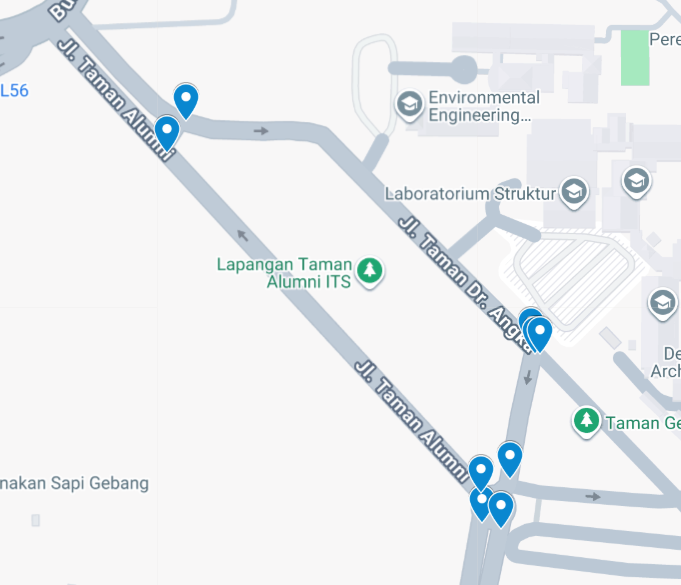
\includegraphics[width=0.5\textwidth]{gambar/google_my_maps.png}
    \caption{Pembuatan rute di Google My Maps}
    \label{fig:google_maps}
\end{figure}

Dari titik-titik yang ditandai, dapat dibentuk segmen-segmen jalan yang menghubungkan titik awal dan titik akhir yang ditunjukkan pada Gambar~\ref{fig:google_segment}.
Segmen ini diekspor dari Google My Maps dalam format KML, kemudian dikonversi menjadi GeoJSON.

\begin{figure}[H]
    \centering
    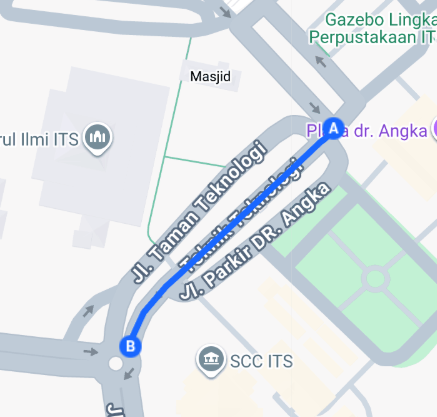
\includegraphics[width=0.5\textwidth]{gambar/google_segment.png}
    \caption{Penentuan segmen pada Google My Maps}
    \label{fig:google_segment}
\end{figure}

GeoJSON tersebut divisualisasikan terlebih dahulu untuk memverifikasi bentuk jalur dan memastikan seluruh segmen telah diekstraksi dengan benar, seperti ditunjukkan pada Gambar~\ref{fig:geojson}.

\begin{figure}[H]
    \centering
    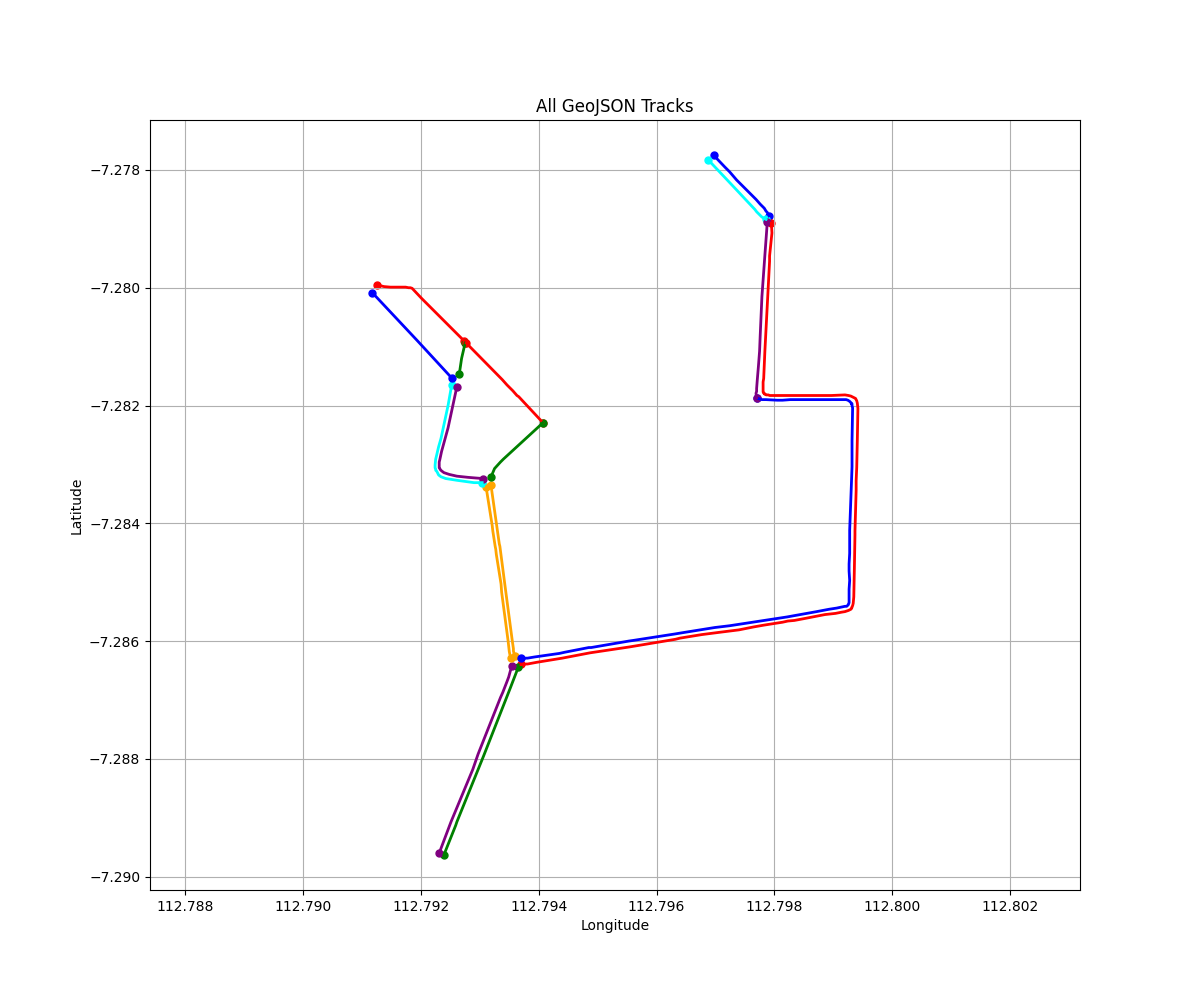
\includegraphics[width=0.75\textwidth]{gambar/geojson.png}
    \caption{Plot segmen GeoJSON}
    \label{fig:geojson}
\end{figure}

Setiap segmen GeoJSON diinterpolasi menjadi \emph{waypoint} dalam file CSV dengan jarak 0,5--1 m antar titik.
Struktur \emph{waypoint} berurutan ini memungkinkan kendaraan mengikuti jalur secara konsisten pada setiap segmen jalan, sebagaimana diilustrasikan pada Gambar~\ref{fig:penjelasan_wp}.
Arah jalur kendaraan ditentukan dari pasangan \emph{waypoint} berurutan pada setiap segmen, sebagaimana ditunjukkan pada Gambar~\ref{fig:arah_wp}.

\begin{figure}[H]
    \centering
    \begin{subfigure}[b]{0.58\textwidth}
        \centering
        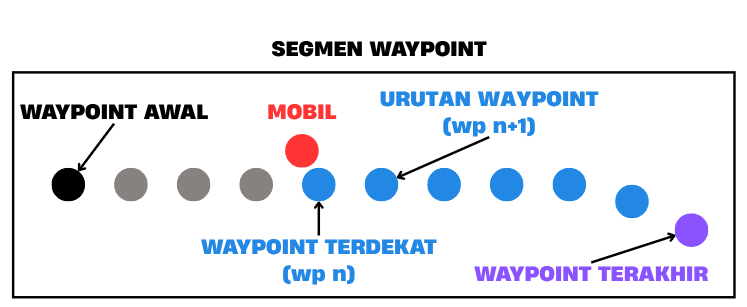
\includegraphics[width=\textwidth]{gambar/penjelasan_wp.png}
        \caption{Penjelasan segmen \emph{waypoint}}
        \label{fig:penjelasan_wp}
    \end{subfigure}
    \hfill
    \begin{subfigure}[b]{0.38\textwidth}
        \centering
        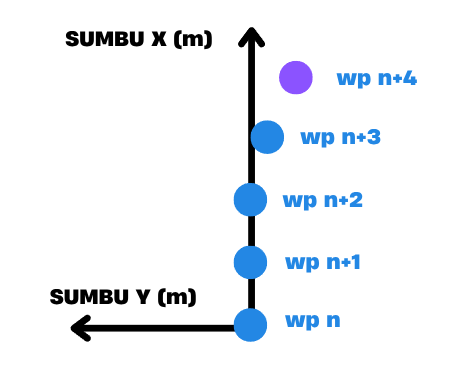
\includegraphics[width=\textwidth]{gambar/arah_wp.png}
        \caption{Penentuan arah dari segmen \emph{waypoint}}
        \label{fig:arah_wp}
    \end{subfigure}
    \caption{Ilustrasi segmen dan arah \emph{waypoint}}
\end{figure}

\subsubsection{Pencarian Rute Global}

Saat sistem diinisialisasi, perencanaan rute global memuat seluruh file CSV \emph{waypoint} dan posisi destinasi.
Dari data segmen yang telah dimuat, dibangun graf berarah dengan aturan dua segmen bertetangga jika jarak antara titik akhir segmen pertama dan titik awal segmen kedua kurang dari 5 m.
Biaya setiap sisi graf ditentukan oleh jumlah \emph{waypoint} dalam segmen tujuan, sehingga segmen yang lebih pendek diprioritaskan oleh algoritma pencarian rute.

Sistem perencanaan rute global berjalan pada frekuensi 10 Hz, di mana setiap iterasi sistem mencari waypoint pada segmen yang memiliki jarak terdekat dari posisi kendaraan saat ini yang dijadikan sebagai titik awal pencarian rute.
Dengan waypoint awal dan waypoint akhir yang sudah ditemukan, dijalankan algoritma Dijkstra untuk mencari rute dengan biaya terendah (jumlah \emph{waypoint} paling sedikit) menuju segmen destinasi.
Kemudian rute yang ditemukan dipotong sejauh 30 m ke depan dari posisi kendaraan saat ini lalu dilakukan transformasi koordinat dari Lat-Lon ke ENU untuk dipublikasikan sebagai rute global dalam kerangka odom.
Sistem juga mengecek apakah kendaraan sudah sampai tujuan, jika jarak kendaraan ke waypoint terakhir kurang dari 1 m, maka sistem menandai rute telah selesai dan menghentikan perencanaan rute global.
Alur kerja perencanaan rute global diilustrasikan pada Gambar~\ref{fig:diagram_navigasi}.

\begin{figure}[H]
    \centering
    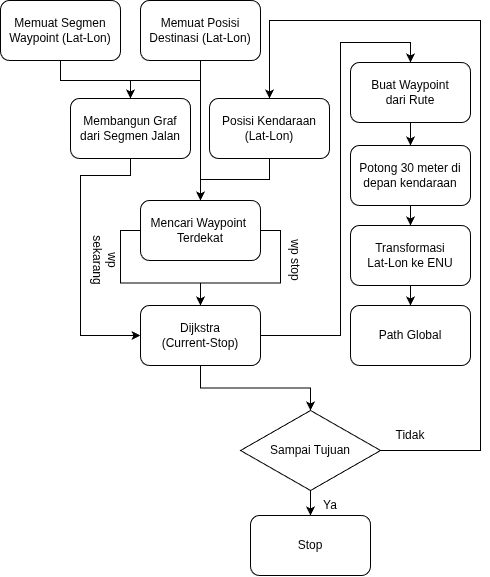
\includegraphics[width=0.8\textwidth]{gambar/diagram_navigasi.png}
    \caption{Diagram alur perencanaan rute global.}
    \label{fig:diagram_navigasi}
\end{figure}

\subsection{Perencanaan Rute Lokal}

\subsubsection{Penyaringan \emph{Obstacle}}

Titik \emph{pointcloud} yang diterima pada tahap perencanaan rute lokal pertama-tama disaring menggunakan informasi rute GPS.
Setiap titik \emph{obstacle} dilakukan pengecekan jarak tegak lurus (\emph{lateral filter}) dari rute global GPS.
Titik yang berjarak lebih dari 5 m dari rute GPS dibuang karena terlalu jauh dengan rute global sehingga dianggap bukan sisi jalan yang sesuai atau valid.
Pemilihan jarak 5 m ini berdasarkan pada lebar jalan di ITS sebesar 6 m, sehingga sisi jalan yang dianggap sebagai titik \emph{obstacle} tetap terdeteksi dengan baik ketika kendaraan berada di tepi jalan.
Visualisasi hasil penyaringan ini ditunjukkan pada Gambar~\ref{fig:obstacle_filtering}.

\begin{figure}[H]
    \centering
    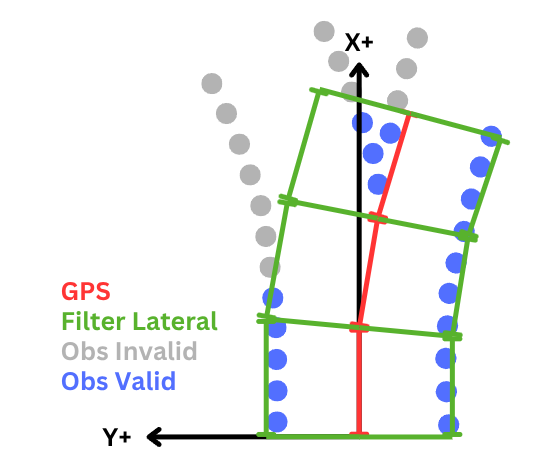
\includegraphics[width=0.5\textwidth]{gambar/filter_lateral.png}
    \caption{Visualisasi hasil penyaringan titik \emph{obstacle} menggunakan informasi rute GPS.}
    \label{fig:obstacle_filtering}
\end{figure}

\subsubsection{Pengelompokan \emph{Obstacle}}

Titik \emph{obstacle} yang hasil penyaringan kemudian dikategorikan menjadi sisi kiri dan kanan jalan.
Proses pengelompokan ini menjadi dua yaitu berdasarkan sudut relatif rute GPS dan batasan jarak lateral (\emph{lateral threshold}).
Pada pengelompokan sudut relatif, setiap titik \emph{obstacle} dihitung sudutnya terhadap arah segmen GPS terdekat seperti yang ditunjukkan pada Gambar~\ref{fig:relative_angle}.
Sudut relatif positif menunjukkan titik berada di sisi kiri jalan, sedangkan sudut relatif negatif menunjukkan titik berada di sisi kanan jalan.

\begin{figure}[H]
    \centering
    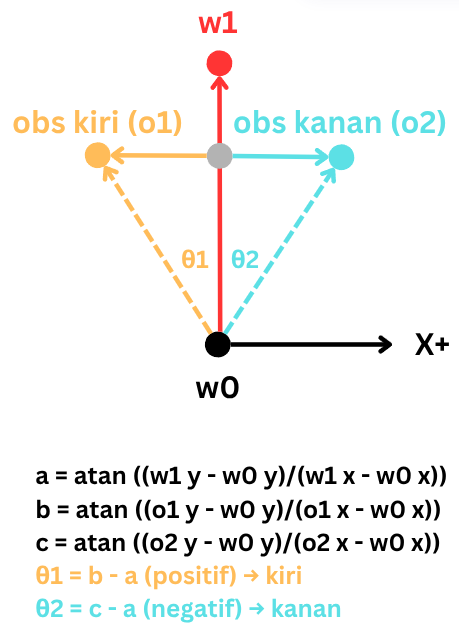
\includegraphics[width=0.45\textwidth]{gambar/kanan_kiri_gps.png}
    \caption{Ilustrasi pengelompokan titik \emph{obstacle} berdasarkan sudut relatif terhadap arah segmen GPS.}
    \label{fig:relative_angle}
\end{figure}

Pengelompokan ini dianggap valid jika kedua sisi masing-masing memiliki minimal 3 titik.
Apabila tidak valid atau titik kurang dari 3, maka sistem beralih ke metode berbasis batasan jarak lateral (\emph{lateral threshold}) untuk mengelompokkan titik.
Pengelompokan berbasis batasan jarak lateral ini menganggap titik valid apabila berada di sisi kanan atau kiri dengan jarak minimal 1,5 m.
Jarak ini dipilih karena lebar kendaraan Omoda E5 sebesar 1,8 m sehingga titik yang berada di luar jarak 1,5 m dianggap sebagai sisi jalan yang valid.
Visualisasi hasil pengelompokan berbasis batasan jarak lateral ditunjukkan pada Gambar~\ref{fig:lateral_threshold}.

\begin{figure}[H]
    \centering
    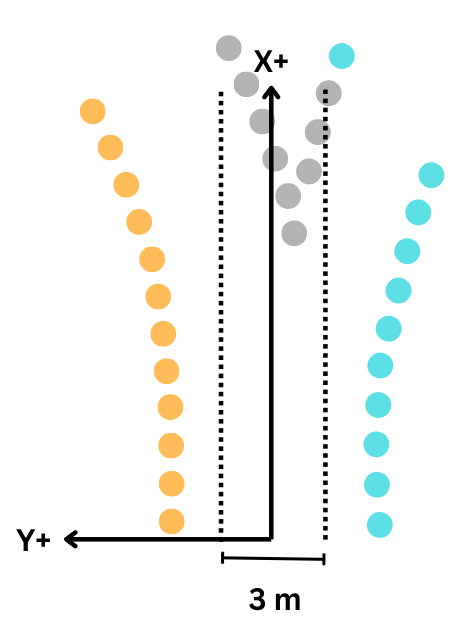
\includegraphics[width=0.26\textwidth]{gambar/kanan_kiri_y.png}
    \caption{Visualisasi hasil pengelompokan titik \emph{obstacle} menggunakan batasan jarak lateral.}
    \label{fig:lateral_threshold}
\end{figure}    

\subsubsection{Pemindaian Titik Tengah Koridor Jalan}

Titik kiri dan kanan yang sudah dikelompokkan kemudian dipindai berdasarkan jendela horizontal untuk menemukan titik kanan dan kiri yang paling dekat dengan kendaraan.
Lebar jendela horizontal ditentukan sebesar 1 m dengan panjang yang mencakup seluruh sumbu y kendaraan.
Titik kanan dan kiri yang terpilih ini akan digunakan untuk menghitung titik tengah koridor jalan yang akan menjadi kandidat titik referensi navigasi.
Titik ini dianggap valid apabila jarak antara titik kiri dan kanan lebih dari 1 m dan kurang dari 10 m, sehingga kendaraan dapat melewati koridor jalan dengan aman.
Jendela akan bergerak ke depan atau sepanjang sumbu x kendaraan untuk menemukan titik kanan dan kiri berikutnya hingga didapatkan titik tengah terakhir atau titik tengah terjauh yang valid.
Visualisasi pemindaian titik kanan dan kiri pada jendela horizontal ditunjukkan pada Gambar~\ref{fig:x_slot_scan}.

\begin{figure}[H]
    \centering
    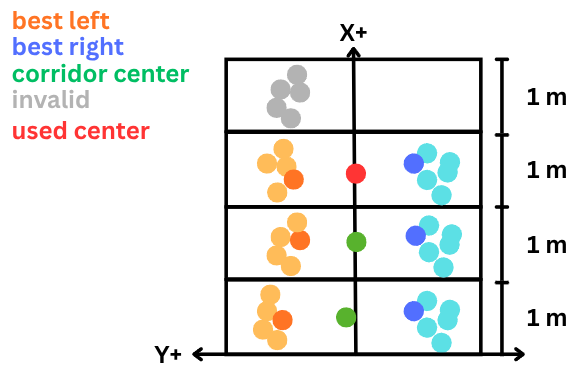
\includegraphics[width=0.45\textwidth]{gambar/best_left_right.png}
    \caption{Ilustrasi pemindaian titik kanan dan kiri pada jendela horizontal.}
    \label{fig:x_slot_scan}
\end{figure}

\subsubsection{\emph{Dynamic Window Approach} Berbasis \emph{Arc Fan}}

Terdapat 3 kemungkinan arah yang dijadikan variabel masukan untuk DWA yaitu berupa sudut kemudi.
Apabila terdapat titik tengah yang valid, maka akan dihitung sudut kemudi referensi dari kendaraan ke titik tengah tersebut.
Jika tidak terdapat titik tengah yang valid, namun masih terdapat rute global GPS, maka sudut kemudi referensi akan dihitung dari kendaraan ke titik acuan GPS terdekat.
Terakhir, jika tidak terdapat titik tengah yang valid maupun rute GPS, maka sudut kemudi referensi akan diatur menjadi 0\textdegree\ untuk mempertahankan arah lurus kendaraan.

Sudut kemudi referensi $\theta_{\text{ref}}$ yang diperoleh dari tahap sebelumnya kemudian divalidasi menggunakan \emph{Dynamic Window Approach} (DWA) berbasis \emph{arc fan}.
Sebanyak 121 kandidat busur dibangkitkan pada rentang $-90$\textdegree\ hingga $+90$\textdegree\ dengan step $1{,}5$\textdegree.
Untuk setiap busur, disimulasikan pergerakan kendaraan selama 2~detik dan diperiksa apakah terdapat \emph{obstacle} dalam jarak \emph{lethal} di setiap langkah simulasi.

Setiap busur $a$ dievaluasi menggunakan fungsi skor yang terdiri dari dua variabel yaitu kedekatan arah terhadap sudut kemudi referensi dan jarak aman kendaraan terdahap \emph{obstacle} sebagaimana didefinisikan pada Persamaan~\eqref{eq:dwa_score} hingga~\eqref{eq:dwa_clearance}.:

\begin{equation}
S(a) = w_h \cdot \exp\!\left(-\frac{|\Delta\theta(a)|}{\theta_s}\right) + w_c \cdot C(a)
\label{eq:dwa_score}
\end{equation}

Fungsi \emph{clearance} $C(a)$ memberikan penalti berdasarkan jarak $d_{\min}(a)$ antara kendaraan dan titik \emph{obstacle} di sepanjang busur $a$.
Jarak bernilai negatif ketika \emph{obstacle} memasuki area kendaraan.
Jika \emph{obstacle} menembus lebih dalam dari toleransi \emph{lethal} $t = 0{,}15$~m ($d_{\min} < -t$), busur diberikan skor $-\infty$.
Jika \emph{obstacle} berada dalam zona penalti ($-t \leq d_{\min} < r$), skor meningkat secara linear dari 0 ke 1.
Jika seluruh \emph{obstacle} berada di luar radius aman $r = 0{,}9$~m ($d_{\min} \geq r$), busur mendapat \emph{clearance} penuh sebesar 1,0:

\begin{equation}
C(a) = 
\begin{cases}
-\infty, & d_{\min}(a) < -t \\
\dfrac{d_{\min}(a) + t}{r + t}, & -t \leq d_{\min}(a) < r \\
1{,}0, & d_{\min}(a) \geq r
\end{cases}
\label{eq:dwa_clearance}
\end{equation}

Nilai $w_h$ adalah bobot untuk kemiripan arah, $w_c$ adalah bobot untuk \emph{clearance} atau jarak aman, dan $\theta_s$ adalah rentang toleransi sudut.
Busur yang memiliki skor tertinggi dipilih sebagai arah navigasi yang optimal, sehingga kendaraan dapat mengikuti rute dengan aman sambil menghindari \emph{obstacle} di sekitarnya seperti yang ditunjukkan pada Gambar~\ref{fig:dwa_evaluation}.
Alur lengkap perencanaan rute lokal diilustrasikan pada Gambar~\ref{fig:diagram_planner}.

\begin{figure}[H]
    \centering
    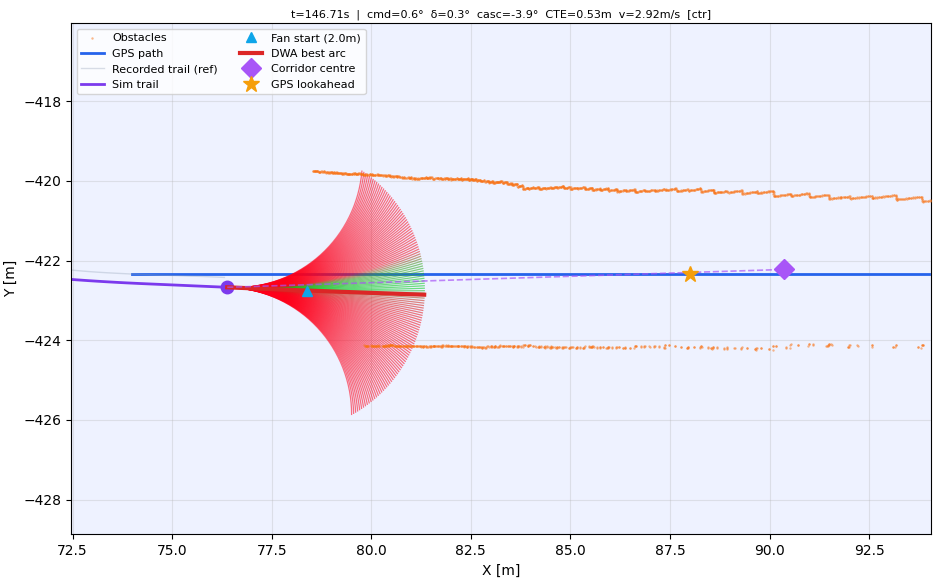
\includegraphics[width=0.5\textwidth]{gambar/dwa_arc.png}
    \caption{Ilustrasi evaluasi busur DWA berbasis \emph{arc fan}.}
    \label{fig:dwa_evaluation}
\end{figure}


\begin{figure}[H]
    \centering
    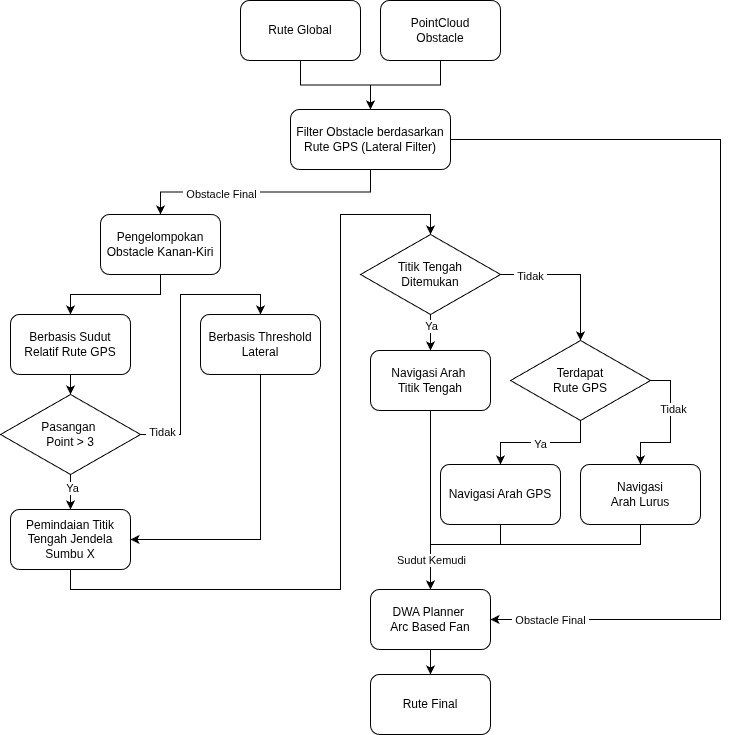
\includegraphics[width=0.9\textwidth]{gambar/diagram_planner.jpg}
    \caption{Diagram alur lengkap perencanaan rute lokal.}
    \label{fig:diagram_planner}
\end{figure}

\subsection{Skenario Pengujian Navigasi}

Pengujian navigasi direncanakan dalam tiga mode operasi yaitu integrasi penuh (\emph{fusion}), hanya segmentasi visual (\emph{vision}), dan hanya \emph{waypoint} GPS.
Selain itu, akan diuji juga skenario dengan injeksi derau pada data GPS untuk mengevaluasi ketahanan sistem terhadap gangguan.
Pengujian dilakukan pada dua rute dengan karakteristik berbeda yaitu rute dengan area persimpangan dan rute dengan tikungan bervariasi.
Setiap mode akan diuji beberapa kali pada masing-masing rute untuk memperoleh data yang representatif.
Selain itu, juga dilakukan pengujian manuver pada jalan lurus, jalan belok, dan bundaran untuk mengevaluasi kemampuan sistem dalam menghadapi berbagai kondisi jalan, serta pengujian \emph{autonomous} pada lintasan jarak jauh untuk mengevaluasi konsistensi sistem dalam bernavigasi secara kontinu.
